\section{Design}
\label{sec:Design}

\subsection{Database Design} 
\paragraph{}The Bmob online database was chosen for the database management system (DBMS) for both the Android application and the web interface because it is a free and open source product that supports the application's required use-cases. 
\par The Bmob cloud storage service platform is a secure and flexible background management system which support 'online database', 'function as a service (FaaS)' and 'game backend cloud service', in our case, we will only use online database. The Bmob cloud storage service platform adopts a multi-tenant virtual isolation mode, that is, any developer's traffic changes or data changes will not affect other developers' applications. 
Another reason to choose Bmob is it supports API interface and multi-language SDK, like Android, IOS, REST API, GO and so on. For our project, we will use both the REST API and the Android API. It supports file uploads and storage,including pictures, videos, audio, and documents. CDN acceleration also makes the upload process faster and more stable but we will mainly use it to upload image files in this project. 
\par The entity relationship (ER) diagram for the whole project is shown in Figure \ref{ERDiagram}.

\begin{figure}[htb]
\centering
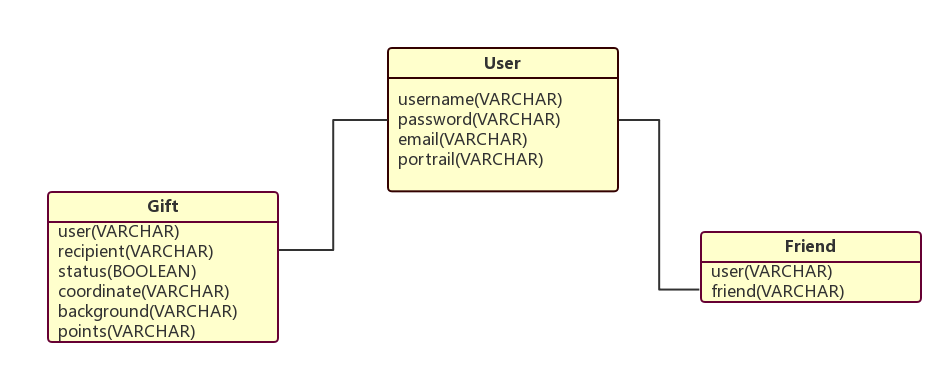
\includegraphics[width=1\textwidth]{section03/assets/ERDiagram.png}
\caption[ER Diagram for the project]{\label{ERDiagram}ER Diagram for the project}
\end{figure}


\begin{itemize}
\item The 'User' table will save all the user information. In this table username and email will be unique for each user and this will be verified when users are registered.
\item The 'Friend' table is for saving all friends pairs and both 'user' and 'friend' columns are usernames from 'User' table.
\item The 'Gift' table saves all the gifts information. The 'user' column records the user who sent the gift. The 'recipient' column records the user who will receive the gift. The 'status' column is a boolean type data meaning the gift is found if it is 'true'. The 'coordinate' column is designed to hold the location where the gift was sent. The 'background' column is designed to hold the region picture. The 'points' column is a string designed to hold the four corners selected by users, it has eight numbers separated by space which means four Xs and four Ys like (x1,y1),(x2,y2) will be saved as "x1 y1 x2 y2".
\end{itemize}

\subsection{User Interface Design}
\paragraph{} We will have two parts for the user interface, one is about the Android application, the other one is for web interface.
\par Following user interface design principles, like accessibility, flexibility, consistency and aesthetics, this user interface is designed to be clear and easy to use. All of pages keep the same color style and use limited colors and fonts so that the user interface is aesthetically pleasing.\cite{galitz2007} 
\subsubsection{Android Application User Interface Design}
\par The main pages for Android application are listed below:
\begin{figure}[htb]
\centering
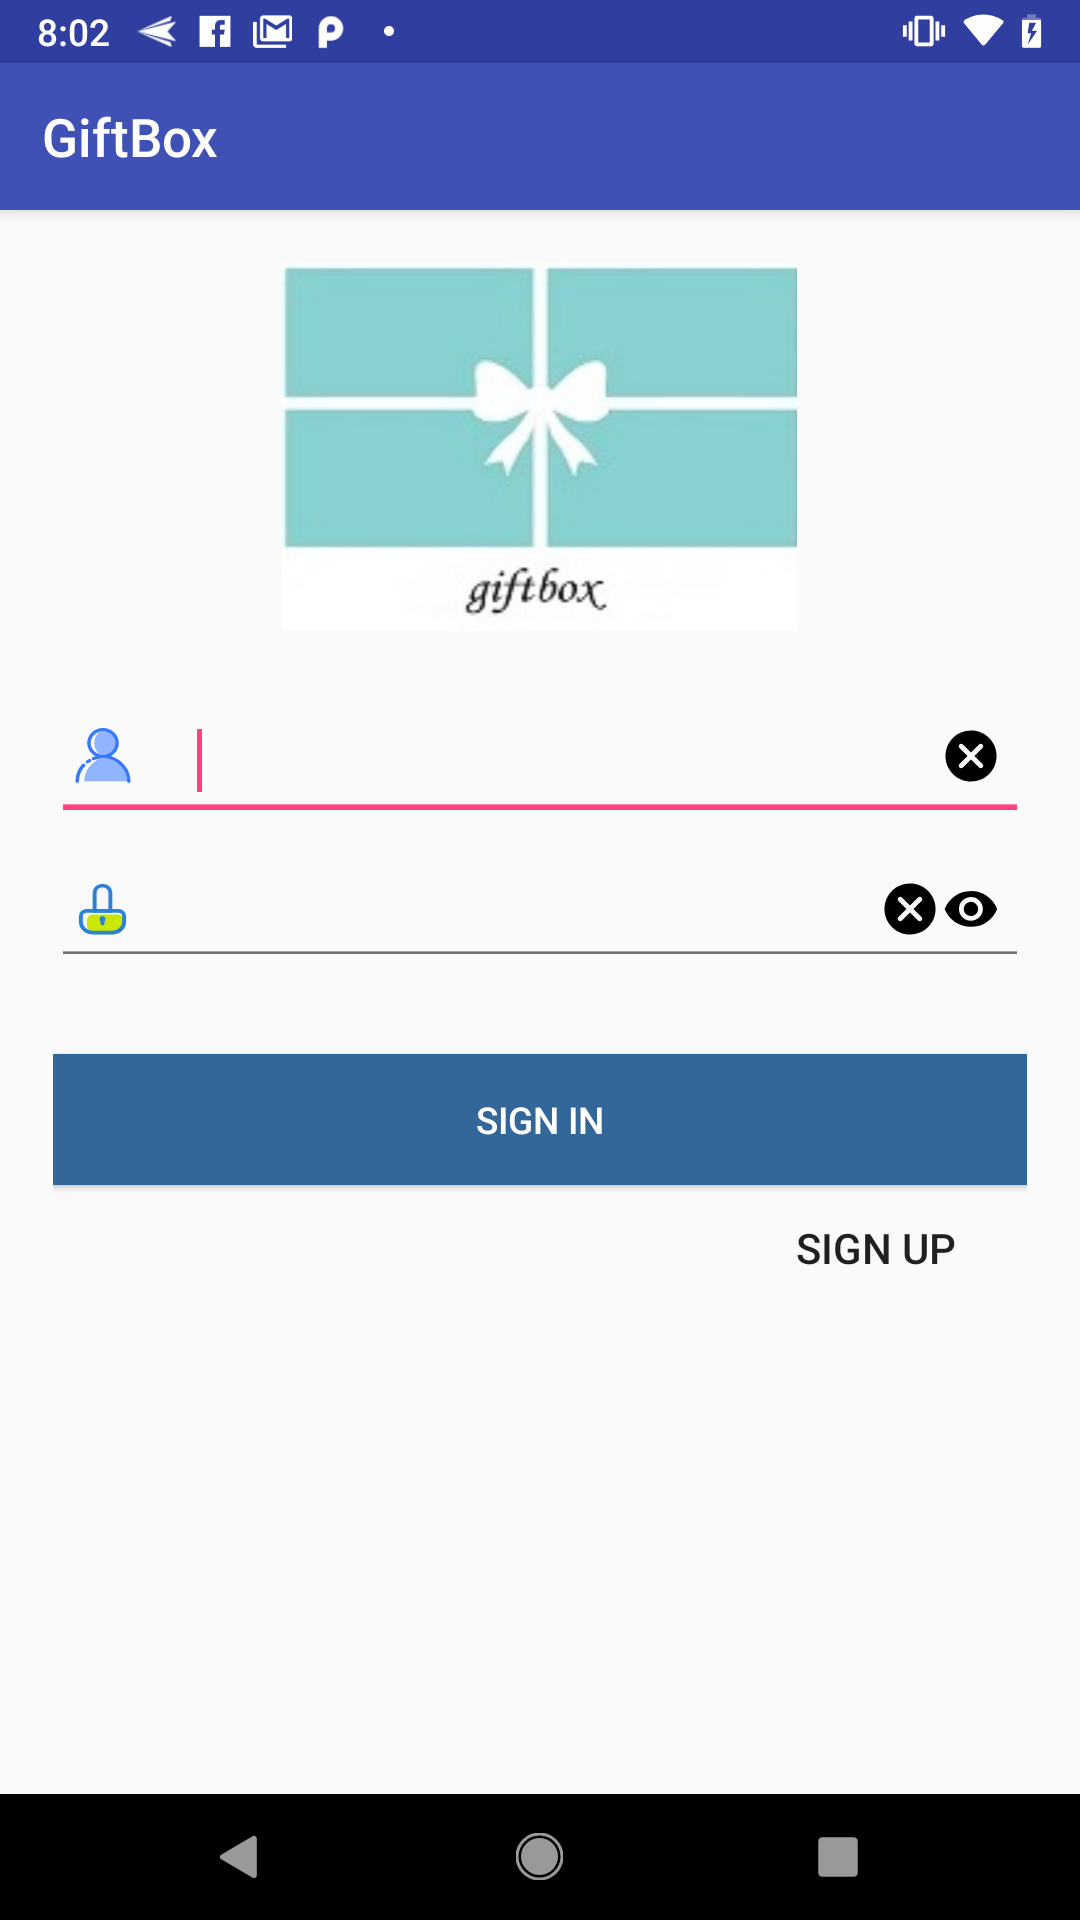
\includegraphics[width=.4\textwidth]{section03/assets/SignIn.png}
\caption[Sign In Page]{\label{SignInUI}Sign In Page}
\end{figure}
\par The sign in page is shown in Figure \ref{SignInUI}. The logo informs users which application they are using. The user icon and the password icon at the left side of the text field hint at the meaning of the two fields to the users. To maintain compatibility, the delete icon and the eye icon at the right side of the text field used another color because they have different functions. Users can use the delete button to clear the text field and use the eye button to view the password in plain text or hidden text.

\begin{figure}[H]
\centering
\begin{minipage}[t]{0.4\textwidth}
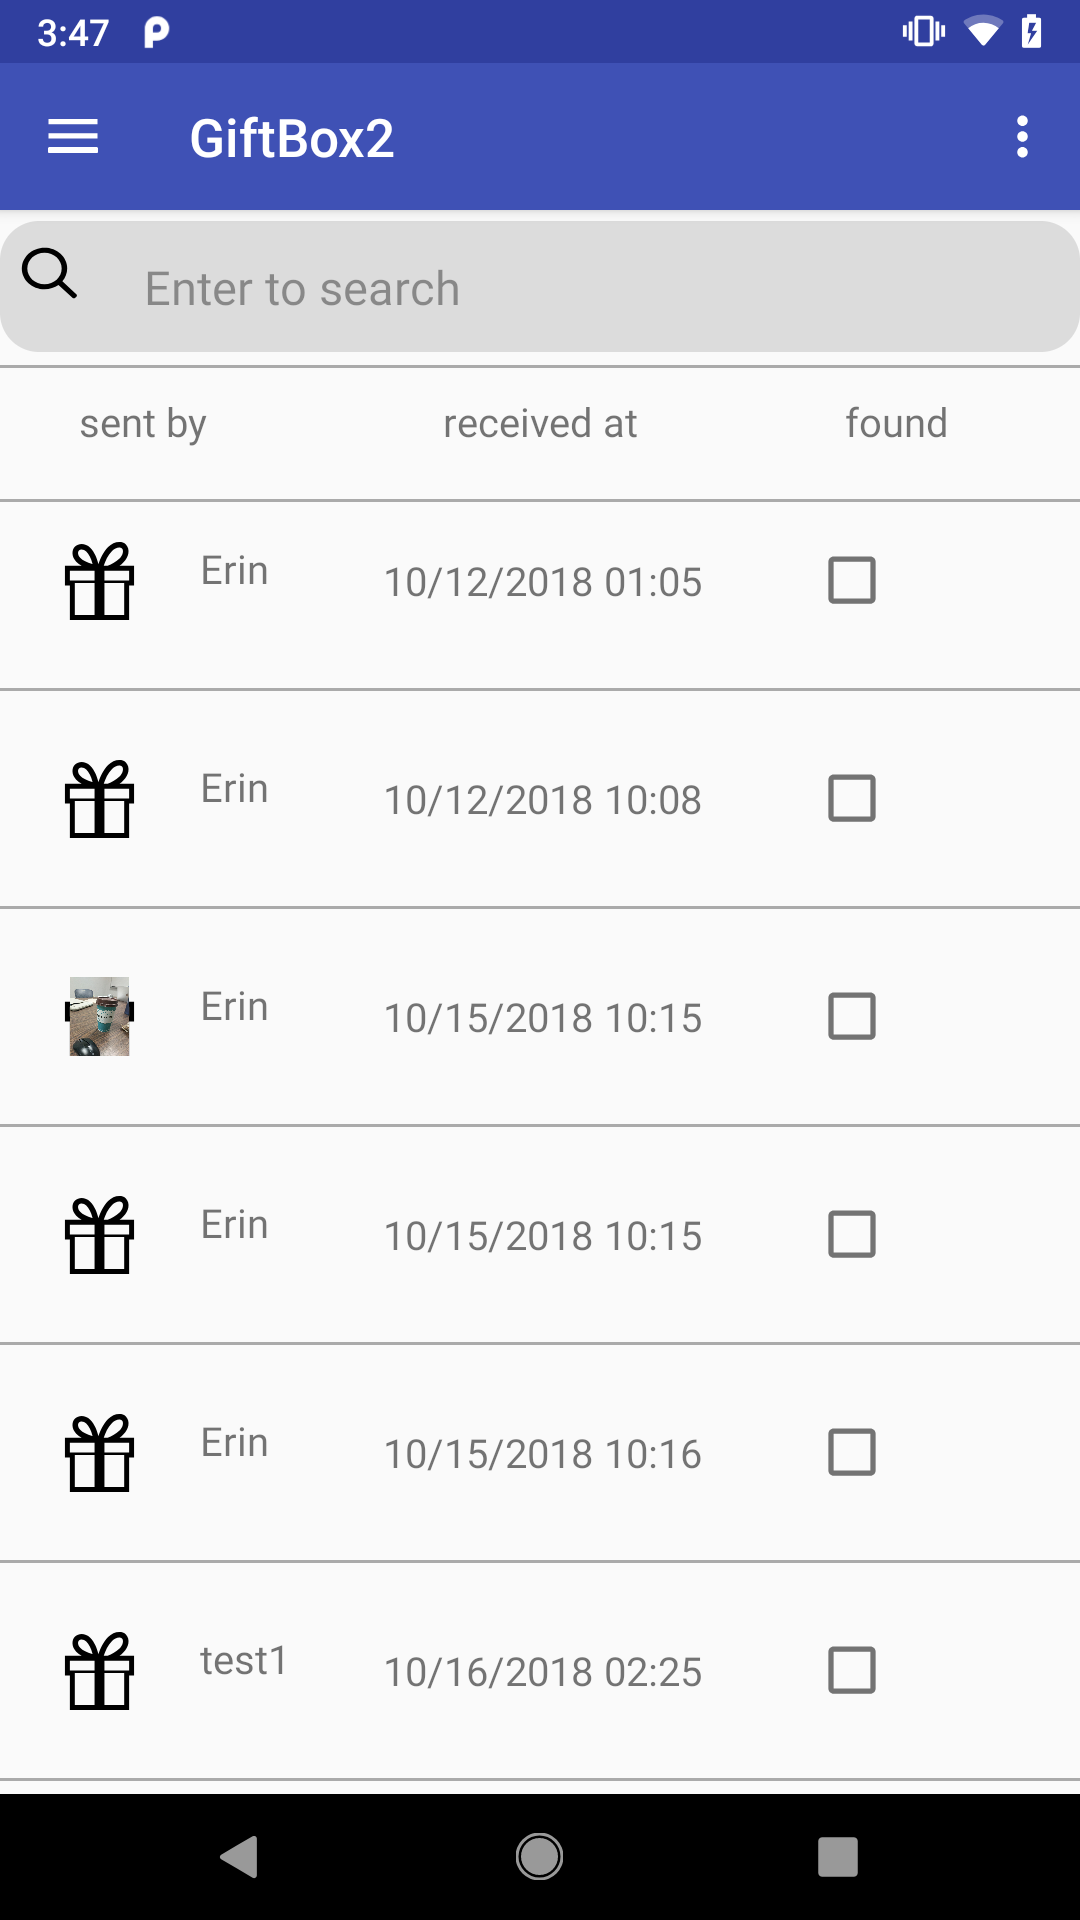
\includegraphics[width=.95\textwidth]{section03/assets/MainPage.png}
\subcaption{\label{GiftsListMainUI}}
\end{minipage}%
\begin{minipage}[t]{0.4\textwidth}
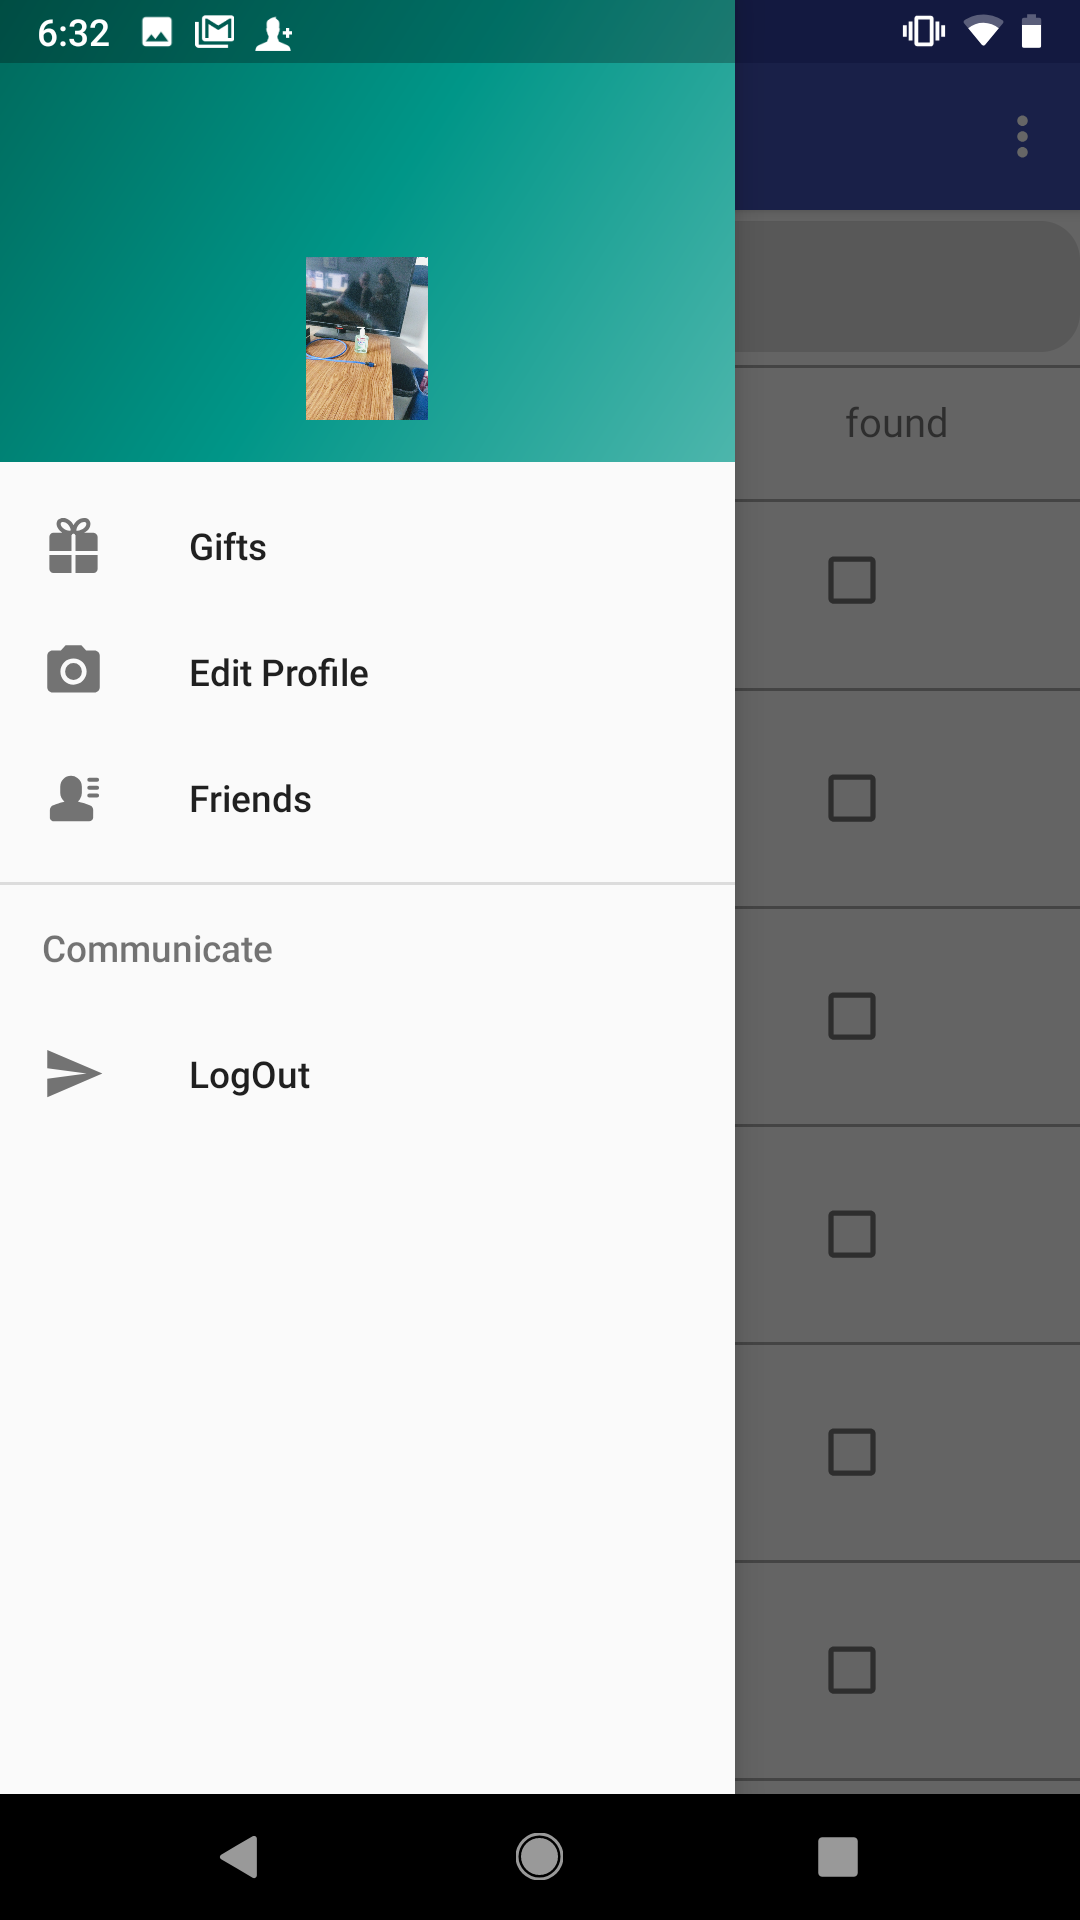
\includegraphics[width=.95\textwidth]{section03/assets/MainPortrait.png}
\subcaption{\label{FunctionsMainUI}}
\end{minipage}%
\caption[Main Page]{\label{MainPageUI}Main Page}
\end{figure}
\par The main page shown in Figure \ref{MainPageUI} will come up after users log in. The main page shows the gifts received by the user. The search field allows users to search by username. This page also has titles to tell users the meaning of each column. The 'gift' icon was replaced by user portraits later. The found column shows whether or not the gift is found. If the 'found' column is checked this means the gift is found.
\par The top left corner navigation menu will lead users to other functional pages. Users will see their portraits on the top of this page and will be able to change their portraits by clicking on the profile picture. They can also view their gifts list by clicking on the 'Gifts' button, edit their profile by clicking on the 'Edit Profile' button, view their friends list as shown in Figure \ref{FriendsListUI} by clicking on the 'Friends' button and they will be able to log out from the system by clicking on the 'LogOut' button. 

\begin{figure}[htb]
\centering
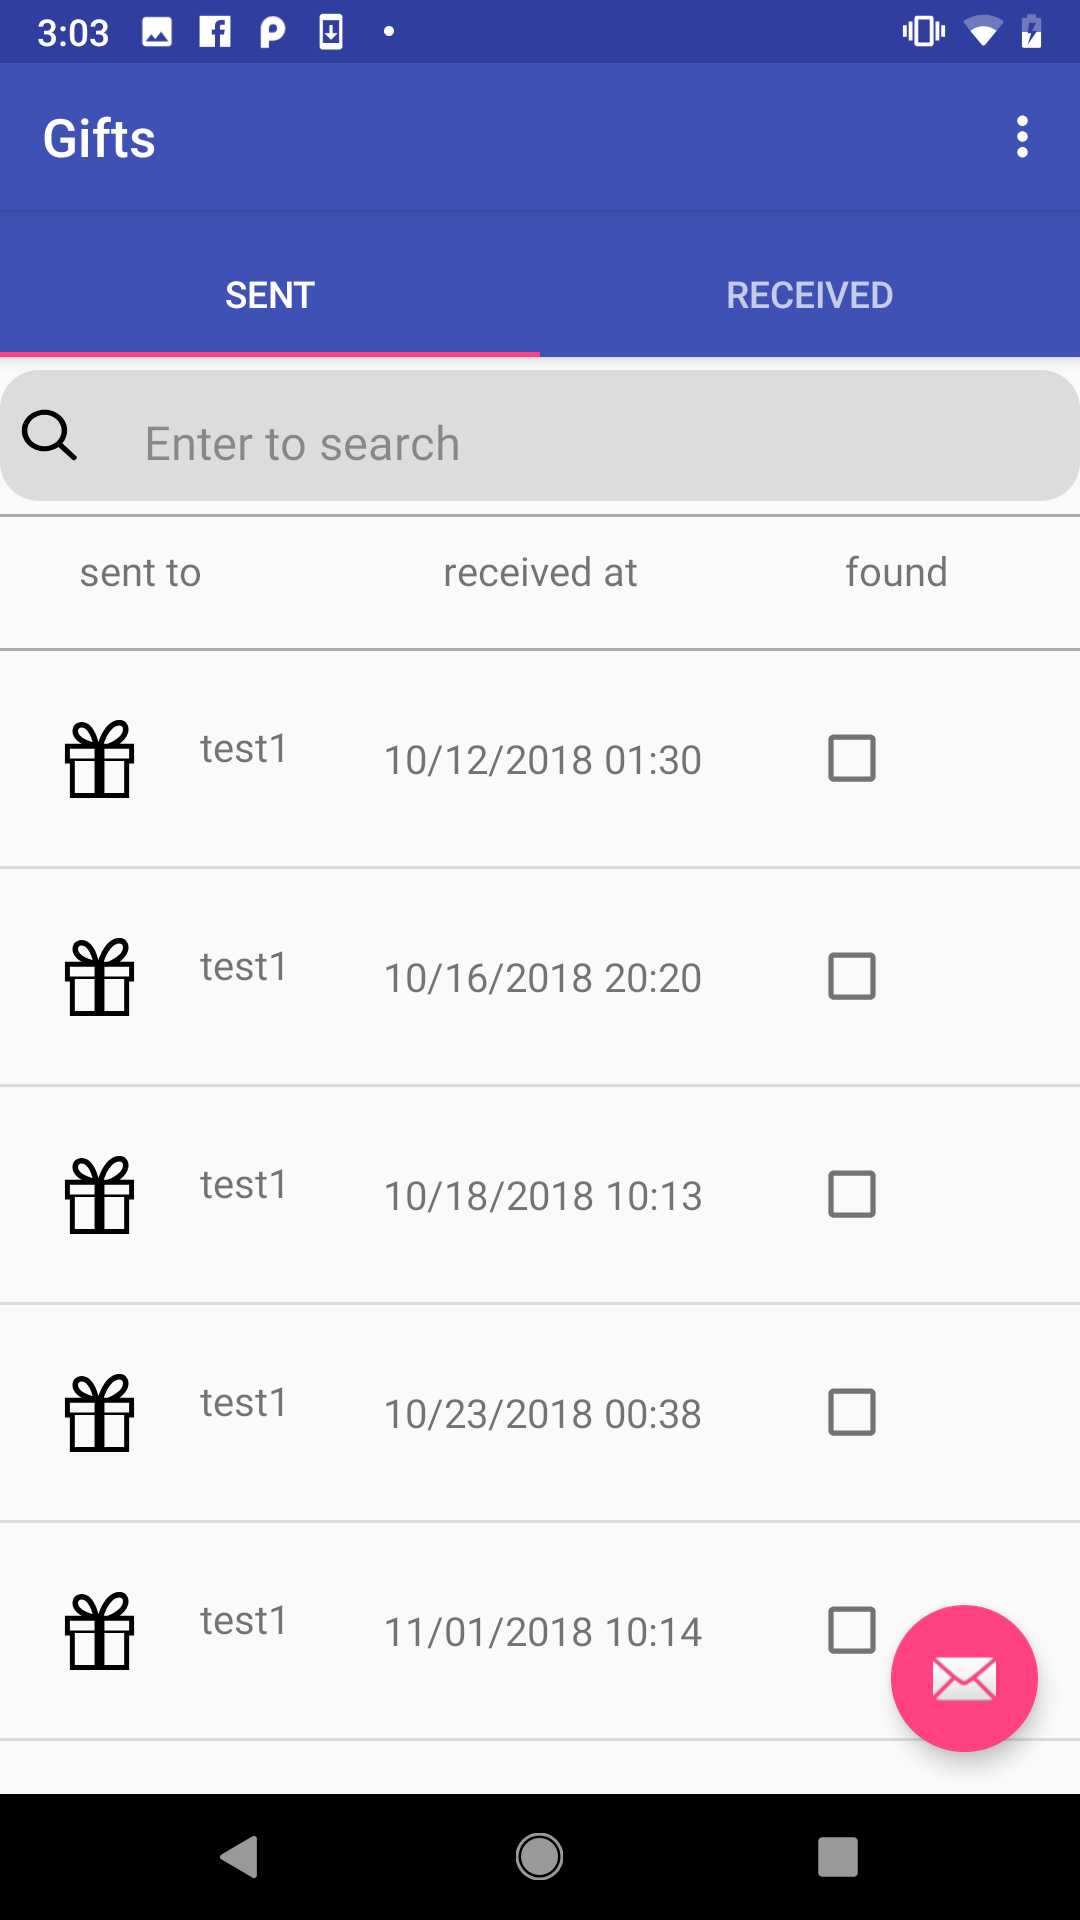
\includegraphics[width=.4\textwidth]{section03/assets/GiftsList.png}
\caption[Gifts List Page]{\label{GiftsListUI}Gifts List Page}
\end{figure}
\par Figure \ref{GiftsListUI}, gifts list page shows the 'gifts list' which is very similar to the main page's gifts list but in this page users will be able to see not only received gifts but also sent gifts ordered by time stamp. For the sent gifts, users will be able to see if this gift is found or not by clicking on the gift. For the received gifts, they can only view found gifts and begin to find unfound gifts by clicking on the gift. 


\begin{figure}[H]
\centering
\begin{minipage}[t]{0.4\textwidth}
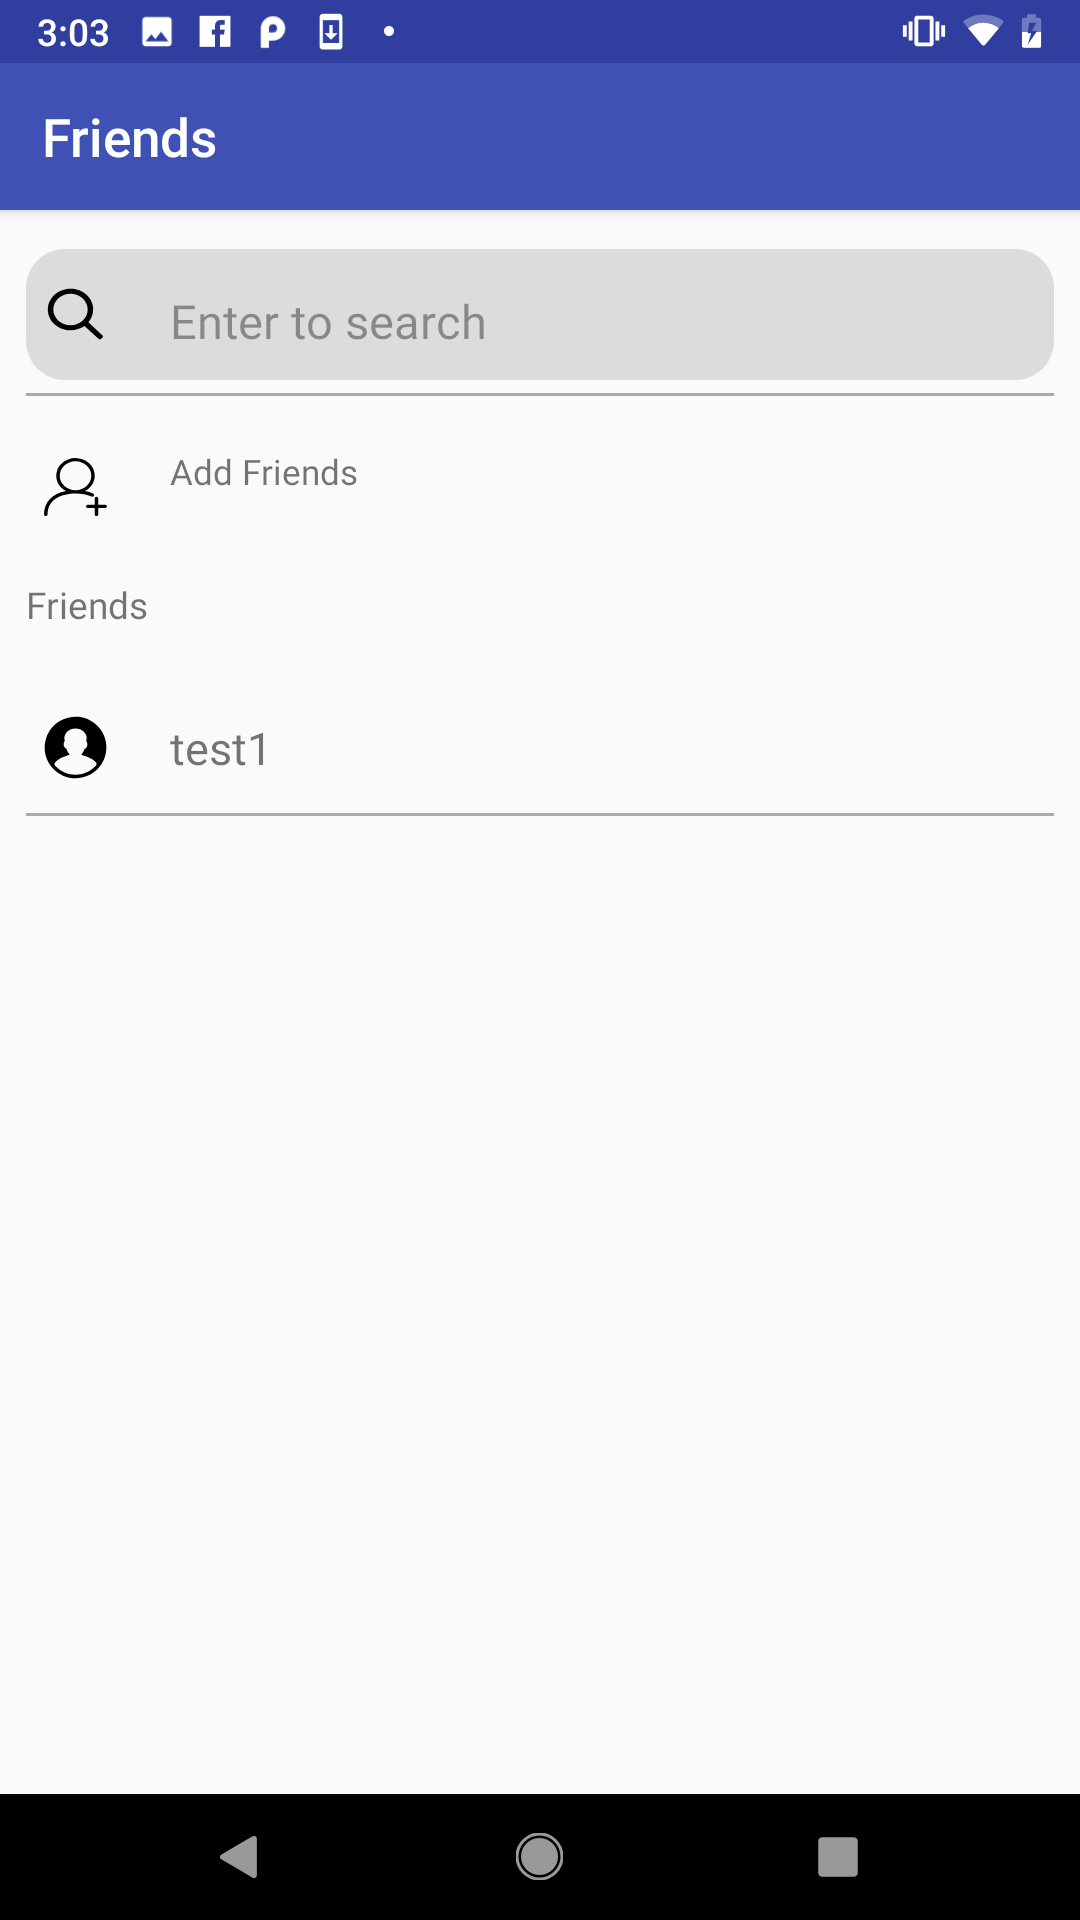
\includegraphics[width=.95\textwidth]{section03/assets/FriendsList.png}
\subcaption{\label{FriendsListUI}}
\end{minipage}%
\begin{minipage}[t]{0.4\textwidth}
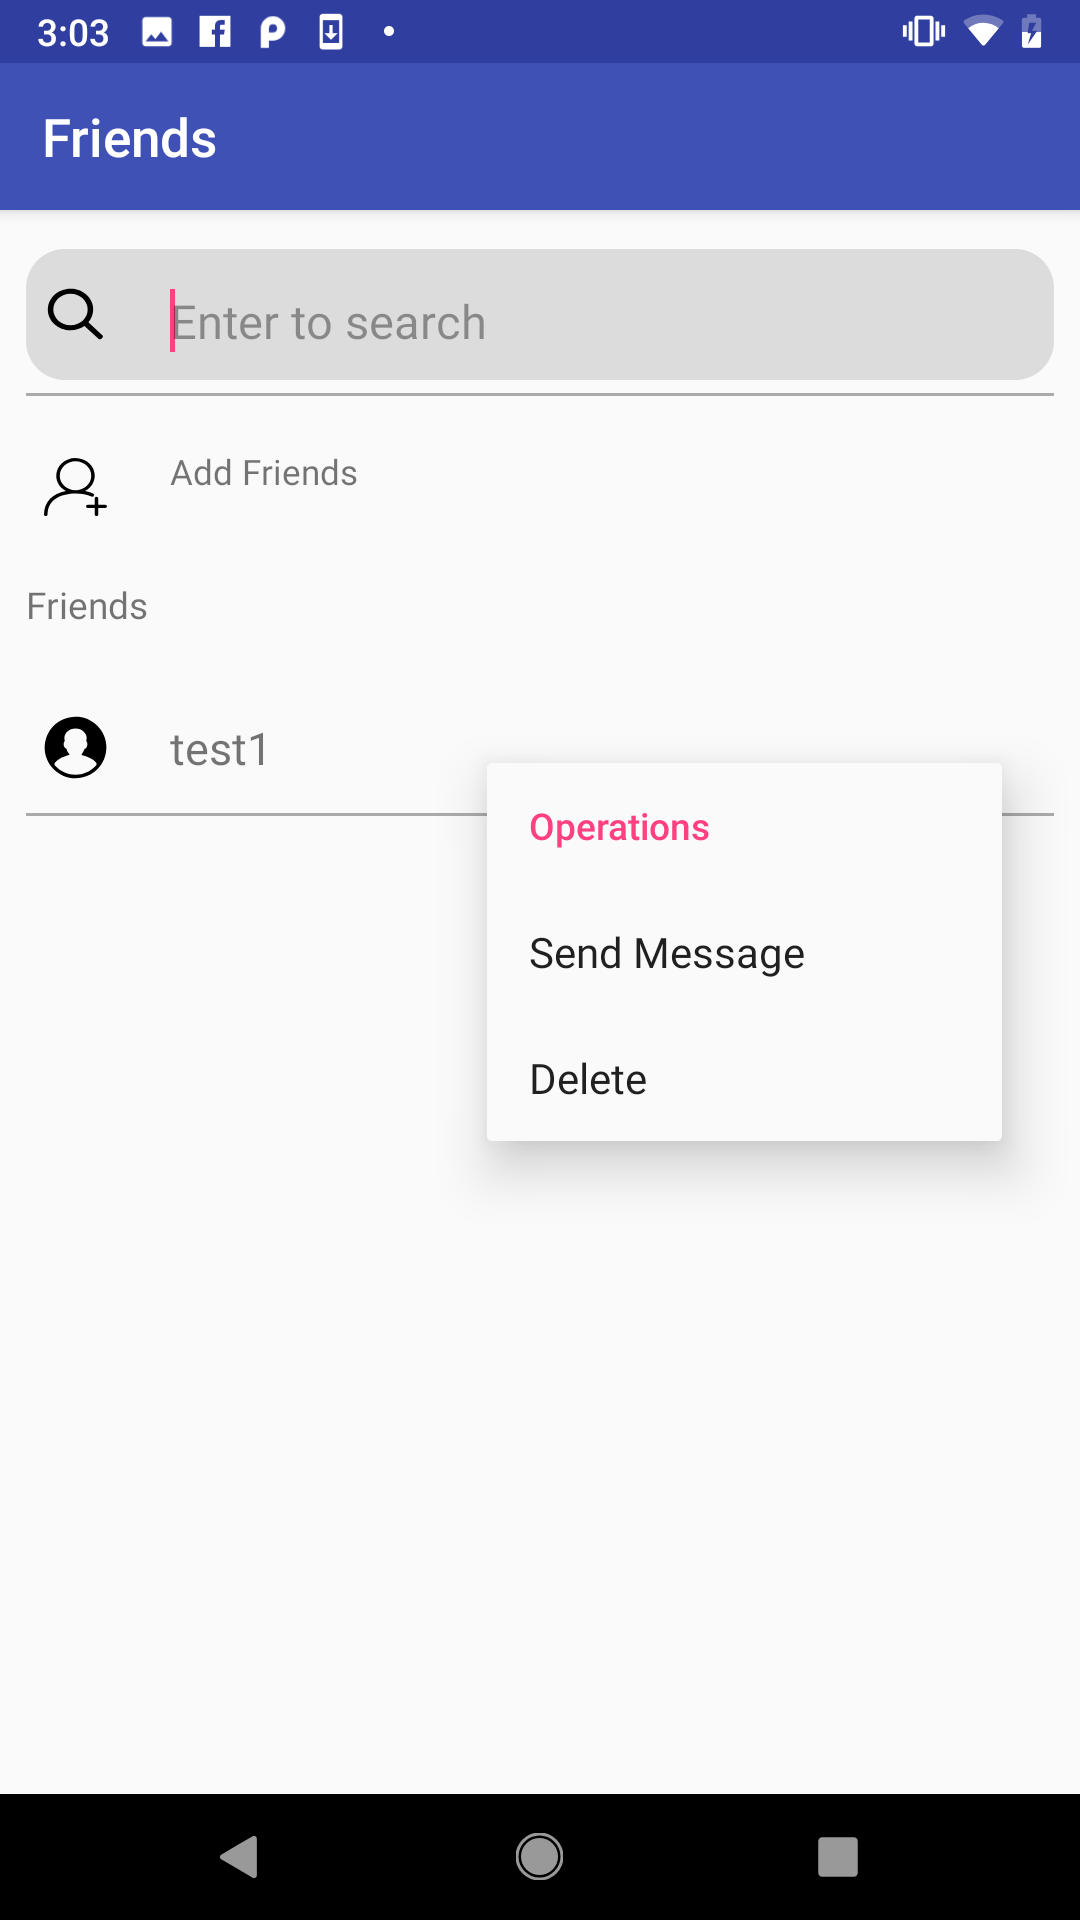
\includegraphics[width=.95\textwidth]{section03/assets/FriendsListAction.png}
\subcaption{\label{FriendsListActionUI}}
\end{minipage}%
\caption[Friends List Page]{\label{WholeFriendsListUI}Friends List Page}
\end{figure}

\par As shown in Figure \ref{WholeFriendsListUI}, the friends list is another important page for this application. To convenience users, the search field can let users search their friends if their friends list is too long. Users can also add friends by clicking on the 'Add Friends' button. The friends list is shown below. Users can get further functions like 'Send Message' and 'Delete' by a long clicking on friends' names, as shown in Figure \ref{FriendsListActionUI}. 

\begin{figure}[H]
\centering
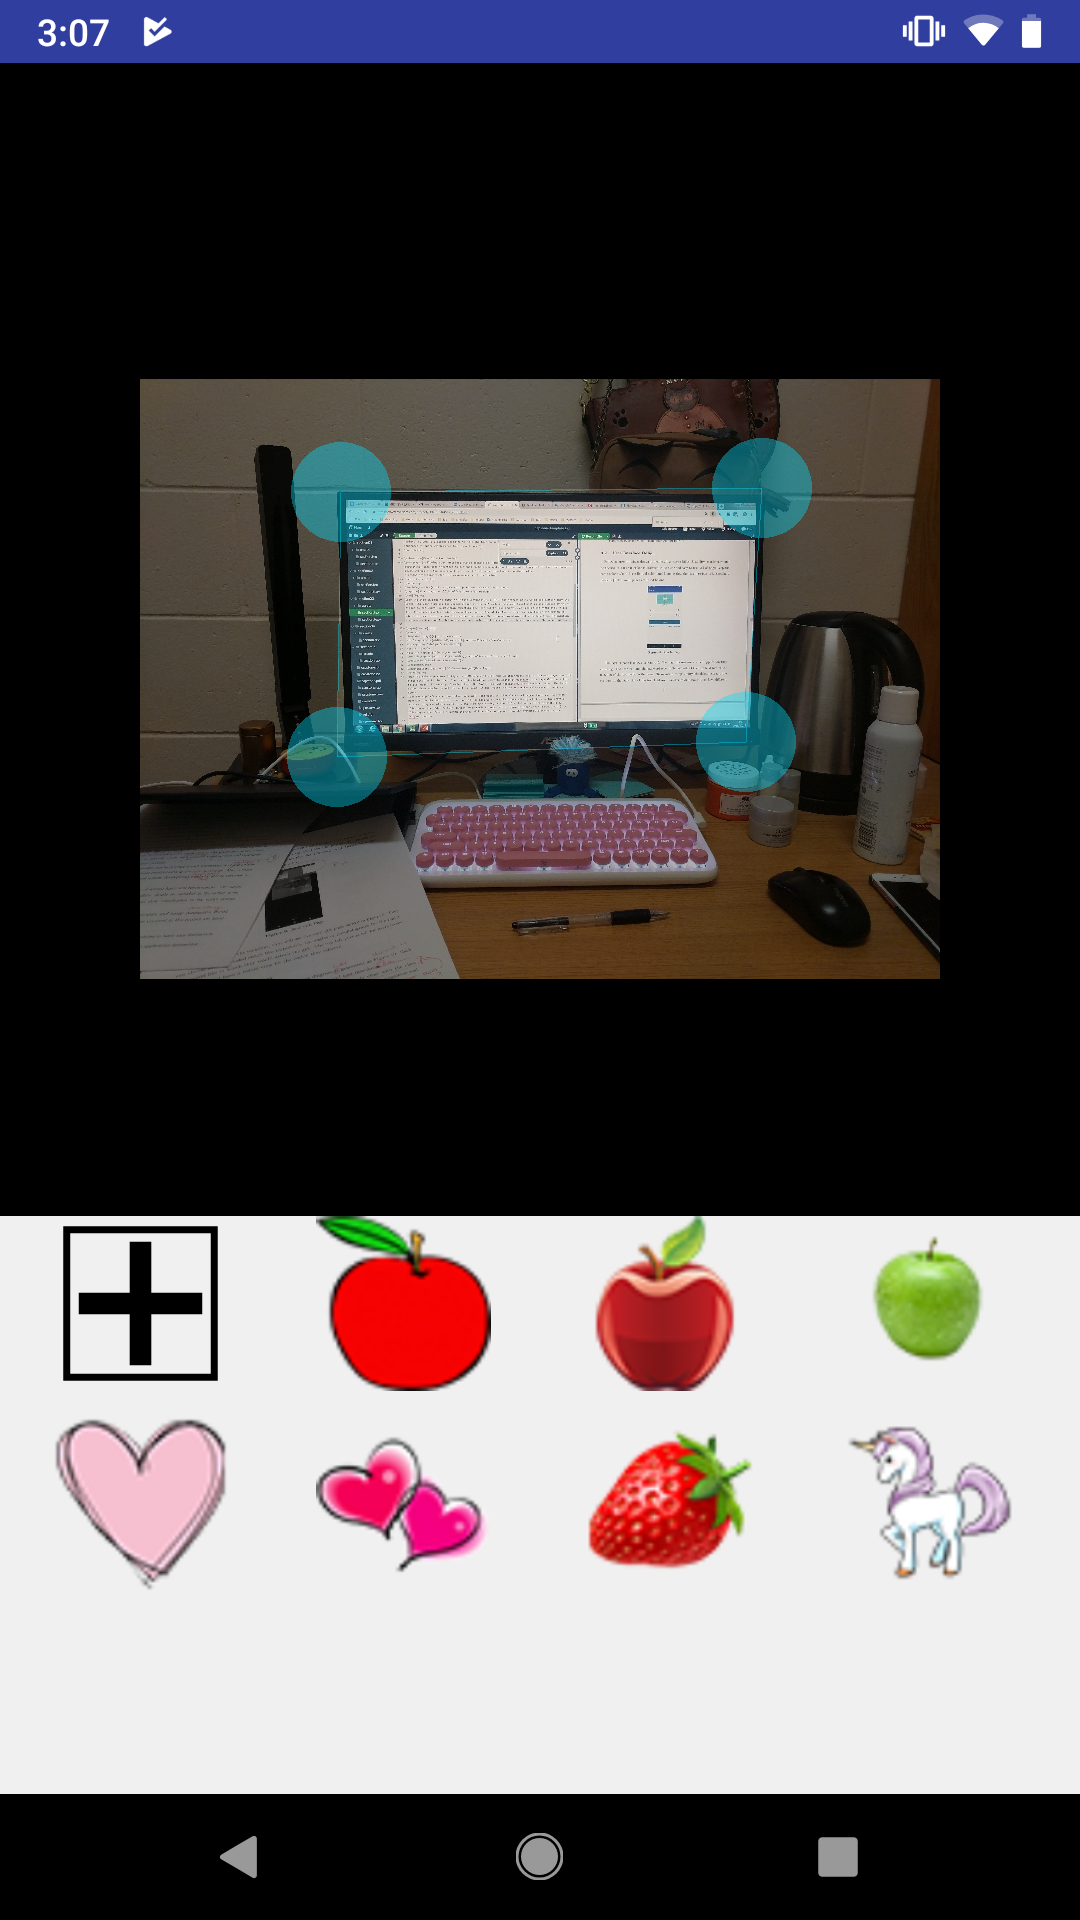
\includegraphics[width=.4\textwidth]{section03/assets/SendGift.png}
\caption[Send Gift Page]{\label{SendGiftUI}Send Gift Page}
\end{figure}
\par After users choose the recipient, they will see the send gift page shown in Figure \ref{SendGiftUI}. They can choose any four sided shape like trapezoids, rectangles or parallelograms for the region they would like in which they would attach the gift. When they finish region selection they will see the gift options at the bottom. Users can choose a gift offered by system or create a new one by taking a picture themselves. 

\subsection{Architecture Design}
\paragraph{}Based on the functional requirements, the class diagram for Android application and the class diagram for web interface was generated shown in Figure \ref{AndroidClassDiagram} and Figure \ref{WebClassDiagram}. Each class corresponds to one or more functional requirements and user interfaces.
\par As we can see, the basic user interaction related activities such as 'log in', 'log out', 'edit profile' and so don't have too many algorithm-related functions. We chose a meaningful name which can quickly shows the purpose of the method, so we don't need any illustration for them. We are just going to explain activities and functions about image recognition and navigation.

\begin{figure}[htb]
\centering
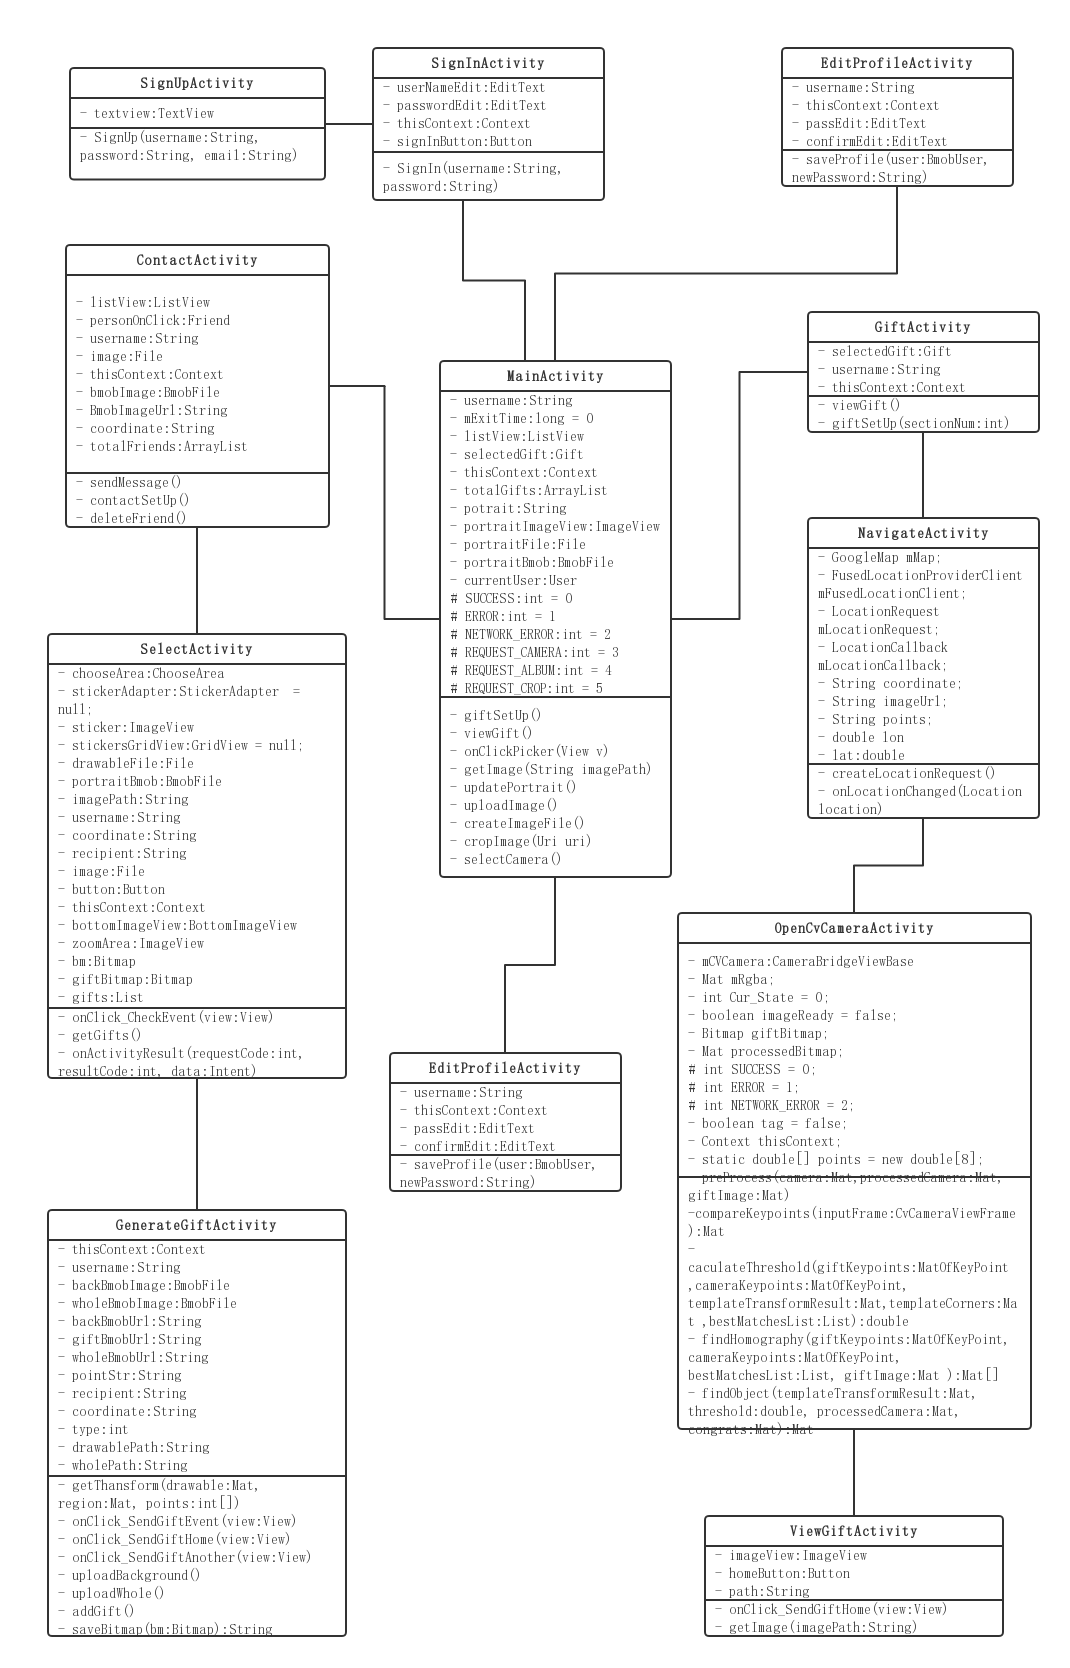
\includegraphics[width=.9\textwidth]{section03/assets/AndroidClassDiagram.png}
\caption[Class Diagram for Android Application]{\label{AndroidClassDiagram}Class Diagram for Android Application}
\end{figure}

\begin{figure}[htb]
\centering
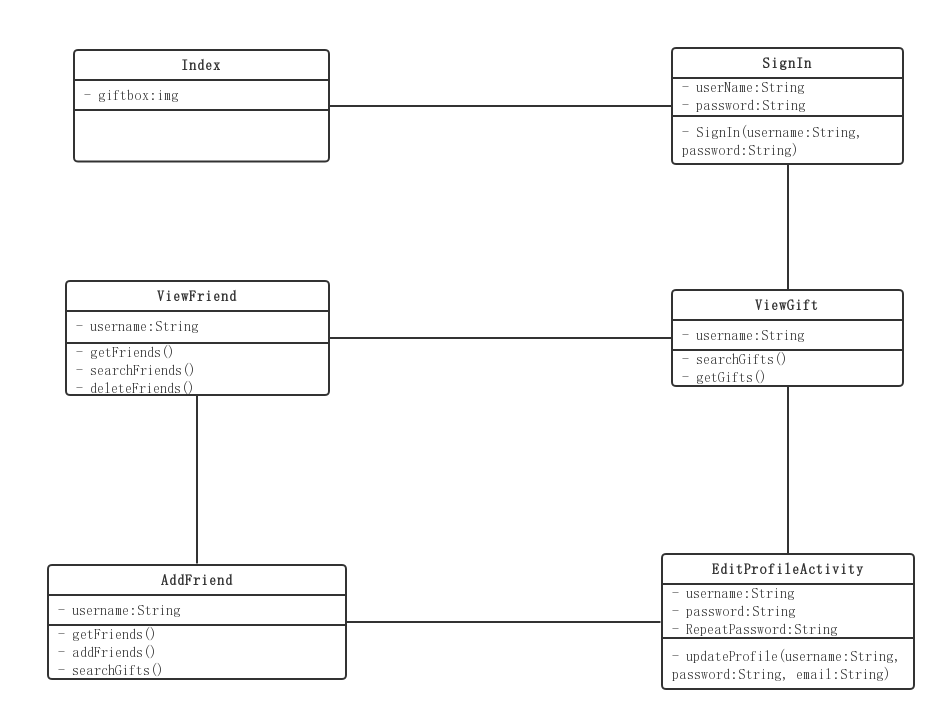
\includegraphics[width=.9\textwidth]{section03/assets/WebClassDiagram.png}
\caption[Class Diagram for Web Interface]{\label{WebClassDiagram}Class Diagram for Web Interface}
\end{figure}
\par The design and implement for web interface is very similar to the Android application and all the functionalities are included in the Android application so we will focus more on the Android Application.
\par The 'ContactActivity' is mainly related to the user interface shown in Figure \ref{FriendsListUI}, users will be able select a recipient and the information will be taken to 'SelectActivity' by an intent and then the system camera will be called to get the background image. The 'chooseArea' attribute is an instance of helper class 'ChooseArea' to let the users choose the region. After that, the gift will fit in the region by 'getTransform' method and 'addGift' method will save all the information to the database.
\par The receiving process is explained as followed. The 'GiftActivity' is designed to show the gift list which is shown in Figure \ref{GiftsListUI}, when users click on a not found gift they will go to 'NavigationActivity'. The 'NavigationActivity' is designed to manage user locations and Google Map activities. Users will be able to see their location on the map and the gift location will be marked as a red point. When users find where the gift locates, the real-time image recognition will start. The camera-captured images will compare with the database saved background image. The 'preProcess' method is used to download the database saved background image and resize the camera-captured images. The 'compareKeypoints' method calculates the keypoints in two images and finds the matches. The 'findHomography' method will use the matches found before to generate the homography and perform a perspective transformation on the template image to correct the image to get the region in camera image. But this method cannot always get the correct result, so the 'caculateThreshold' method calculates the value of the number of keypoints not in the selected region divided by the number of keypoints in detected region, this value will be later used as a threshold to determine if the region we found is good. At last, the 'findObject' method will get the final detected region and show the gift on it.

\subsubsection{The Web User Interface Design}
\paragraph{} The web interface is mainly used to retrieve data from the database and show them in a user readable way. So we designed the web interface like shown below:
\begin{figure}[htb]
\centering
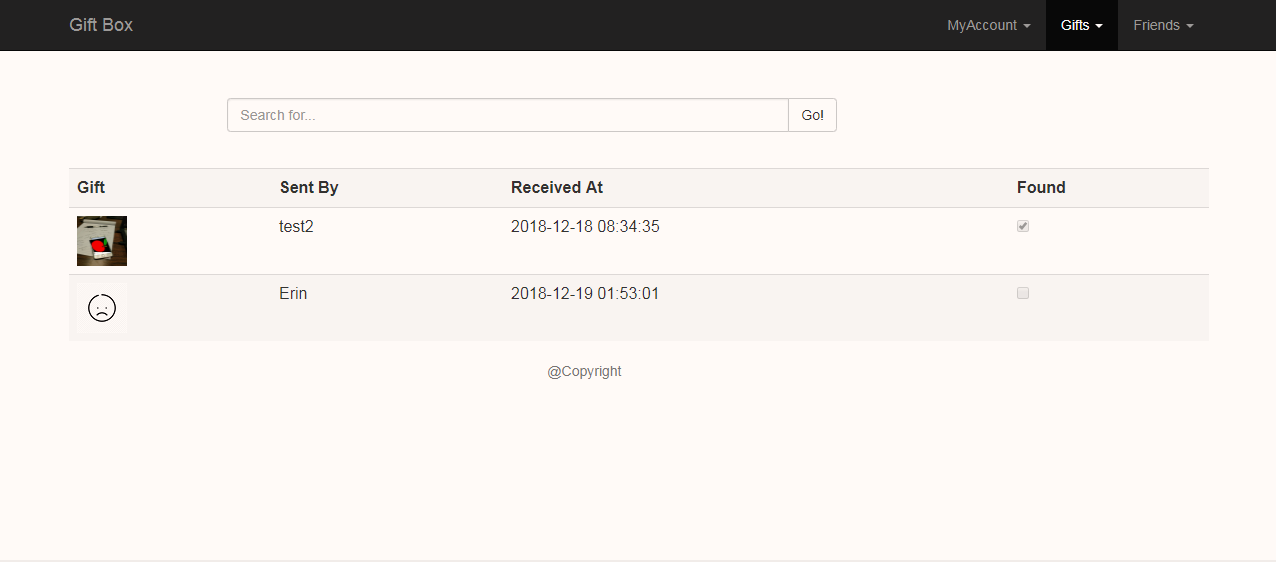
\includegraphics[width=.9\textwidth]{section03/assets/ViewGifts.png}
\caption[View Gift Page for Web Interface]{\label{ViewGift}View Gift Page for Web Interface}
\end{figure}
\par The view gift page designed similar to the 'gifts list page' in Android so that user will feel familiar and that will be easy for a user to use another application if they used one before. In Figure \ref{ViewGift} View Gift Page, users will only be able to see the received gifts which is found and an unhappy face at the gift column will show up if the gift is not found. Users can also search their gifts list by username.

\begin{figure}[htb]
\centering
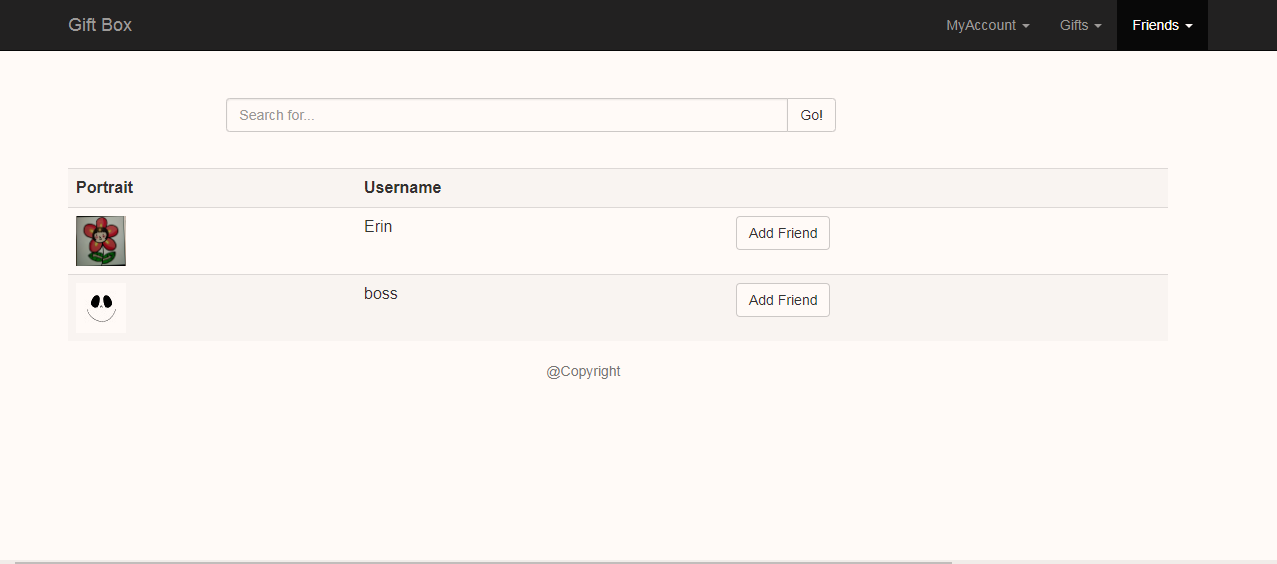
\includegraphics[width=.9\textwidth]{section03/assets/AddFriends.png}
\caption[Add Friend Page for Web Interface]{\label{AddFriends}Add Friend Page for Web Interface}
\end{figure}
\par As shown in Figure \ref{AddFriends} Add Friend Page, all the users which are not currently friend will be listed. Users can search by user name if there are too many users in that page.